\documentclass[report]{jsbook}
\usepackage[dvipdfmx]{graphicx}
\usepackage[dvipdfmx]{color}
\usepackage{booktabs}
\usepackage{latexsym}
\usepackage{okumacro}
\usepackage{fancybox,ascmac}
\usepackage{sty/algorithm}
\usepackage{sty/algorithmic}
\usepackage{colortbl}
\usepackage{multirow}
\usepackage{listings}
\usepackage{sty/jlisting}
\usepackage{url}
\usepackage{amsmath}
\usepackage{amsfonts}
\usepackage[noreplace]{otf}
\lstset{
	language={Java},
	basicstyle={\small},
	breaklines={true},
	frame=tRBl,
	framesep=5pt,
}

\newcommand\figref[1]{図\ref{#1}}
\newcommand\tabref[1]{表\ref{#1}}
\newcommand\equref[1]{式\ref{#1}}

\setcounter{tocdepth}{2}

\begin{document}
\pagestyle{empty}

\begin{center}

\vspace{5cm}

\textbf{\Large 卒業論文~2020年度(令和2年度)}

\vspace{2cm}

\textbf{\LARGE Depth2Jam:ドライブレコーダーを用いた渋滞推定システム}

\vspace{3cm}

\textbf{\underline{\large 指導教員}}\\
\textbf{慶應義塾大学環境情報学部}

% \textbf{\Large 徳田~~英幸}\\
\textbf{\Large 村井~~純}\\
\textbf{\Large 楠本~~博之}\\
\textbf{\Large 中村~~修}\\
\textbf{\Large 高汐~~一紀}\\
%\textbf{\Large 重近~~範行}\\
%\textbf{\Large 湧川~~隆次}\\
\textbf{\Large Rodney D. Van Meter III}\\
\textbf{\Large 植原~~啓介}\\
\textbf{\Large 三次~~仁}\\
\textbf{\Large 中澤~~仁}\\
\textbf{\Large 武田~~圭史}\\
%\textbf{\Large 加藤~~貴昭}\\

\vspace{6cm}

\textbf{\LARGE 慶應義塾大学 環境情報学部}

\vspace{.5em}

\textbf{\LARGE 李 広耀}

\vspace{.3em}

\textbf{\it koyo@ht.sfc.keio.ac.jp}

\newpage

\end{center}

\pagestyle{plain}

\frontmatter
\begin{center}
\textbf{\Large 卒業論文要旨 2019年度(令和元年度)}

\vspace{6.18mm}

\textbf{\Large ドライブレコーダーを利用した渋滞推定システム}
\end{center}

\vspace{10mm}

\begin{flushleft}
\textbf{論文要旨}\\
\end{flushleft}
日本における渋滞情報は主に道路に設置されているセンサーや監視カメラの映像等からリアルタイムに算出されており,自動車のナビゲーションシステム等で使われている.
しかし現状渋滞情報を取得できるのは高速道路や国道といった一部の交通量が多い道路に限られている.
本研究では,近年のドライブレコーダー搭載数の増加や映像技術向上を生かし,ドライブレコーダーから得られる単眼カメラ映像から渋滞推定を行うことで,全ての道路での渋滞推定を可能にすることを目指す.
実装にはドライブレコーダーから得られる単眼カメラ映像を用いて,距離推定ライブラリ及び物体検出システムを利用し,先行車との距離をもとに渋滞しているか否かを推定する.
本研究が実現すると,現在のVICS等の渋滞,交通量を検知,測定するシステムでは賄えないような,細い道,住宅街の道,一方通行など,さまざまな道路で突発的に発生した渋滞情報を共有することができる.


\begin{flushleft}
\textbf{キーワード}\\
\textbf{ドライブレコーダー,渋滞,深層学習,画像処理}

\end{flushleft}

\begin{flushright}
\textbf{慶應義塾大学 環境情報学部}\\
\textbf{李 広耀}
\end{flushright}
\newpage



\setlength{\baselineskip}{13pt}
\begin{center}
\textbf{\large Abstract of Bachelor's Thesis Academic Year 2020}

\vspace{6mm}

\textbf{\large Depth2Jam : Congestion Estimation System Using a Drive Recorder}

\end{center}

\vspace{10mm}


\begin{flushleft}
\textbf{Abstract}\\
\end{flushleft}
In Japan, traffic jam information is mainly obtained from sensors and monitoring cameras installed on roads, and sent to traffic information management centers such as VICS, which in turn send the information to car navigation systems.
However, traffic jam information can currently be obtained only on some roads, such as expressways and national ways, and cannot be collected on other roads.
In addition, the installation rate of drive recorders has been increasing as a result of recent improvements in performance and the surfacing of dangerous and incendiary driving.
However, there are few cases in which the videos from the installed drive recorders are used for viewing.
Since the drive recorder is a video device, it can collect various data by detecting objects and recognizing images.
The purpose of this research is to propose a new way to use the drive recorder and reducing the area where traffic jam information can be collected, which is limited.
As an approach to the purpose, we propose Depth2Jam, a system to estimate traffic jam from the images of drive recorders.
In this study, we implemented Depth2Jam and conducted an experimental evaluation of the accuracy of traffic jam estimation.
In addition, we show the improvement of the accuracy of Depth2Jam and its future prospects.

\begin{flushleft}
\textbf{Keywords}\\
\textbf{Drive Recorder,Traffic Jam, Deep Learning, Image Processing}
\end{flushleft}

\begin{flushright}
\textbf{Keio University Faculty of Environment and Infomation Studies.}\\
\textbf{Koyo Ri}\\
\end{flushright}


\setlength{\baselineskip}{16pt}
\tableofcontents
\listoffigures
\listoftables

\mainmatter
\chapter{はじめに}
本章では,はじめに本研究における背景とその目的等について述べる
\section{背景}
% 背景と問題----------
日本はアメリカや中国などの道路と比較して国土が狭く、人口密度が高い。それに伴って車道が狭く、渋滞が起こりやすくなっており、日々テレビやラジオのニュースで渋滞情報が報道されている。

%渋滞を減らすことを目指すのではなく、渋滞を推定することのメリットについて語るべきかもしれない。-----

日本では、渋滞情報は、VICS等の企業が道路に設置されているセンサーや車道付近に置かれているカメラの映像、および自動車に搭載されているセンサーやGPSの情報などをもとに算出されている。
また、日本におけるカーナビゲーションシステムはVICS等の渋滞情報を元に到着予想時刻などを割り出している。
加えて、渋滞情報はGoogle社が提供しているGoogle Mapにも提供されており、Web上でリアルタイムのデーターを閲覧することが可能である。
しかし、VICS等が管理している渋滞情報は、国道や高速道路といった日常的に交通量が多い道路には設置されているが、そうではない細い道や一方通行といった道では渋滞情報がない。

%煽り運転の話------------軽く
また近年、煽り運転等のマナーの悪い運転が報道されるようになり、伴って各自動車へのドライブレコーダー搭載数が年々上昇している。
ドライブレコーダーは走行中の記録を撮ることにより事故の時の証拠を残すことができると同時に、事故等の証拠にもなり、警視庁も交通安全の面で、ウェブサイトにおいて取り付けを推奨している。
元々、煽り運転等の危険運転はドライブレコーダーが登場する前から発生していたが、近年社会問題として取り上げられているのはドライブレコーダーやスマートフォンなど、映像技術の向上により人々が気軽に高画質な映像を録画、記録することが可能になったからである。
加えて近年のSNSの普及により、一般の人でも容易に事故の動画を発信したりと、注意喚起を行うことが可能になった。
結果、煽り運転のような危険運転が容易に可視化され、ドライブレコーダーや、スマートフォンで撮影した映像がニュースでも取り上げられるようになった。
このような社会的変化を考えれば、ドライブレコーダーを単純な映像記録装置として扱うのでは不十分であり、さまざまな機能をつけることで、より効果的、効率的に扱えるようになると言える。

\section{目的}
%この研究の目指すところについて述べる----------軽く
本研究の目指すところは、入力された画像および動画から、走行している場所が渋滞しているか否かを判断することにある。
加えて、本研究が目指すものは、渋滞の判断、評価のプロセスの次のフェーズとして、渋滞している場合、実際に渋滞している現場の画像及び映像をサーバーにアップロードすること、さらにその後のフェーズとして、ドライバー同士でそのような渋滞情報を共有することである。
交通の安全上、ドライバーは運転中にカーナビ等の電子機器を操作することは禁止されているため、システムが渋滞だと判断した場合、自動で渋滞データをアップロードする必要があり、また、渋滞データーはオープンな情報としてドライバーに共有される必要がある。
%以上の2つのフェーズを最終的に加えることで、このシステムの本来目指しているものは完成する。

\section{ドライブレコーダーについて}
現在、一般的なドライブレコーダーは単なる記録装置として活用されているが、ドライブレコーダーの映像からは先行車や道路の状態、歩行者など、さまざまなデータを取得することが可能であり、様々な事象を可視化することができることが考えられる。
本研究ではドライブレコーダーを使用して渋滞を推定することで、VICSやGoogle Map、そしてGPSの情報だけではでは見ることができない道路の渋滞の現場を可視化することを目的とする。
VICSでは車両感知器(Vehicle Detectors)と光学式車両感知器の2つが主に使われ、それぞれ通過車両台数や渋滞情報を自動的に感知し交通管制センターへ送信する役割と、通過車両を感知するとともに車載装置との双方向の通信を行う役割を持っている。
さらに、VICSは主に国産の自動車メーカーに取り付けられているカーナビゲーションシステムで主に利用されているため、外国産の車など、自動車によってはカーナビゲーションシステムがVICSに対応していない例もある。
そして、VICSは日本でのみ使われているシステムであるのに対し、ドライブレコーダーはどのような自動車でも追加で取り付けることが可能であり、渋滞推定を行うことができれば、日本に限らず世界中の道路で渋滞推定を行うことができる汎用性がある。

% 関連研究----------
% 渋滞の定義

\section{渋滞の定義}
渋滞についての研究を行うためには、まず渋滞とはどのような状態か定義する必要がある。
普段我々がニュース等で情報を得ている渋滞情報として、日本道路交通情報センター(JATIC)は、高速道路では、時速40km以下で低速走行あるいは停止発進を繰り返す車列が、1km以上かつ15分以上継続した状態であるとし、一般道では、時速10km以下で低速走行している状態が渋滞であると定義している。
本研究では正確な速度をカメラ映像から割り出すことは不可能なため、それらの定義とは異なる独自の定義を使用する。
%この研究で使っているGoogle Tensorflowが開発したStruct2depthシステムは画像及び動画のデーターを処理し、黄色と藍色の色の濃淡で距離を割り出している。
%カメラと位置が近ければ近いほど黄色い色が濃くなり、カメラから遠ざけば遠ざかるほど藍色の色が濃くなる。この研究では以上の状況を踏まえ、出力された画像及び映像から黄色い色の濃さの割合から先行車との車間距離を推定し、そこから速度を概算し、渋滞かどうか評価する。
%渋滞の定義においては、車道の自動車の数や交通量よりも走行速度の方に焦点が当たっている。


% 研究手法 でもここは別のところに書いた方がいいかもしれない


% 手法の工夫----------
% この工夫のパートが長すぎるかな...

% 実験----------

% 構成----------


\chapter{現在の渋滞に関する問題}
% Tanimu先輩"具体的に都市の画像を用いた想定している有効活用の方法について話す.軽く"
% 俺の研究の場合どんな問題について語ればいいんだろうねよくわからん
% 多分渋滞についての問題を書けばいいのかもしれない(適当)
ここでは本研究をするにあたって、本研究が意識する問題について述べる。

\section{渋滞についての問題点}

\chapter{関連研究}
%ドライブレコーダーを用いた関連研究について
\section{ドライブレコーダーを用いた研究}
自動車にカメラ及びドライブレコーダーを取り付けて行なった研究として,まず道路のひび割れや塗装の剥がれといったものを検出する研究\cite{全邦釘2017ディープラーニングおよび}がある.
画像処理技術が向上したことで,道路における障害物やひび割れといったものの検出が可能となった.
しかし,道路のひび割れのような不動で固定的なものとは異なり,渋滞というものは時間と共に発生したり解消したり,また規模も大きくなったり小さくなったりと変化するものあり,変化するものに対しての画像認識の対応は困難なものだった.

ドライブレコーダーと機械学習を組み合わせたものとしては,Japan Taxi株式会社が既にタクシーに高性能なドライブレコーダーをつけて,走行中の道路の状況等をリアルタイムに収集し解析するというサービスを行なっている.
しかし,そこで行われているのは歩行者の検出や道路工事の検出などであり,発展して渋滞を推定すると言う旨の実現には至っていない.
各タクシーから集められた情報をもとに人間の手で渋滞かどうか判断しているので,本研究によってその人間の判断を自動化する,あるいは事前に渋滞かどうか疑わしい現場の映像に判断材料を絞ることができる点で,本研究には貢献できる点があると言える.

%車載カメラからの画像処理について書きたい
\section{ドライブレコーダー以外の車載カメラを用いた研究について}
ドライブレコーダー以外の車載カメラの研究について,三上ら\cite{三上量弘2020deepcounter}は,ゴミ収集車にカメラ取り付けるとこで,ゴミ収集車にどれほどのゴミ袋が収集されたかを調べる研究を行った.
ゴミ清掃車は,日々決まったルートを通り,決まった場所でゴミを収集している.
その収集されるゴミの量を数値として可視化することで住民の生活の変化を可視化する研究である.
自動車にカメラを取り付けて,映像情報からデーターを可視化するという目的の点で,可視化するデーターが異なるとはいえ,三上らの研究はこの研究と共通点がある.
また,三上らの研究には私の研究と同様のYOLOと呼ばれる物体検出システムが使用されており,その物体検出システムが検出したゴミ袋の量を計測していた.

以上を踏まえると,物体検出システムを使用することでデーターの可視化が可能であると言える.

\newpage

\section{渋滞推定の研究について}
ドライブレコーダー以外の方法でカメラから渋滞を測定する方法として,進藤ら\cite{進藤瞭2013車載カメラ画像を用いた対向車線の渋滞状況の把握手法}は,対向車の交通量を測定することで渋滞を推定する研究を行なった.
進藤らの方法は自動車2台を走行させ,その2台の横を通過した対向車の数から渋滞しているか否かを判断するものである.
しかし,進藤らの方法では測定するための自動車は常に道路の右側車線を走行しなければならないと同時に,対向車道がない道路では渋滞を推定することができないという問題がある.

\section{カメラを用いた距離推定の研究}
%センサー情報を含めた先行研究
車間距離を推定するフェーズに関して,動画から距離を推定する方法はいくつか存在する.
まず最も簡単かつ確実な方法は複眼カメラと三角関数を利用した方法である.
同じ対象を移したときに2つの視点からそれぞれのカメラから対象の距離を測定する方法である.
しかし,本研究の対象はドライブレコーダーであり,1つの自動車に2つのドライブレコーダーを搭載することは現実的ではなく,複眼のドライブレコーダーは一般的に搭載されていないためこの方法は利用できない.
そのため,この研究では単眼カメラの映像から車間距離を推定する必要がる.
単眼カメラから物体との距離を推定する研究としては,カメラ情報に加えて各種距離センサーの情報を利用することで実現する方法が一般的であった.

% Struct2depth
しかし,近年ではDeep Learning技術の向上により,各種センサーといった教師データーのない,純粋に画像のみでの距離推定プログラムが実現している.
Zhouら\cite{zhou2017unsupervised}はセンサー情報等の教師データのないカメラ映像から奥行きを推定するシステムを開発した.
Zhouらのシステムは,車載動画等の連続的な画像の集まりであるデータセットを元に映像における視界の変化を元に奥行きを推定するものであった.
Zhouらの研究以降,カメラ映像における奥行きの研究は,Zhouらの研究を元に性能向上がなされ,Yinら\cite{yin2018geonet}などによってアップデートがなされた.

中でも,Googleの研究チームのCasserらが行なった研究である"Struct2Depth"\cite{casser2019struct2depth}というシステムは上記の研究と比較して精度がより向上されている\figref{fig:depth_related}.
本研究ではStruct2Depthを利用し,車間距離を推定する.

\newpage

\begin{figure}[hp]
  \begin{center}
   \includegraphics[width=\textwidth]{figs/struct2depth_related.png}
  \end{center}
  \caption{struct2depthと他の研究の比較\cite{casser2019struct2depth}}
  \label{fig:depth_related}
\end{figure}

\begin{figure}[hp]
  \begin{center}
   \includegraphics[width=\textwidth]{figs/aproach_depth.png}
  \end{center}
  \caption{struct2depthのアプローチ(https://sites.google.com/view/struct2depth)}
  \label{fig:approach_depth}
\end{figure}

\newpage
\section{物体検出システムについて}
%YOLOとかの話
物体検出を行うライブラリは様々あり,Fast R-CNNs\cite{ren2015faster},Mask R-CNN\cite{he2017mask},SSD\cite{liu2016ssd}といった手法が挙げられる.
それぞれCNNと呼ばれる畳み込みネットワークを利用し物体検出を行なっている点は同じだが,CNNの層や物体検出を行う際の手法がわずかながらに異なっている.
本研究では物体検出手法としてYOLO(You Only Look Once)\cite{yolov3}\figref{fig:yolo_system}\figref{fig:yolo_network}と呼ばれる物体検出手法を用いる.
YOLOは上記の3つの手法と比較して畳み込みネットワークやニューラルネットワークがシンプルな構造になっているにもかかわらず,高い検出率を誇っている.
また,構造が比較的シンプルなため演算処理にかかるスピードが速く,リアルタイムでの処理にも適している.
本研究では,YOLOがMicrosoft COCO datasetを機械学習したものを利用し,ドライブレコーダーに写っている自動車,トラック,バスを主に検出させ,距離推定及びその結果からシステムの評価を行う.


\begin{figure}[htbp]
  \begin{center}
    \includegraphics[width=\textwidth]{figs/Yolo_Detection_system.png}
    \caption{YOLOの物体検出システム\cite{yolov3}}
    \label{fig:yolo_system}
  \end{center}
\end{figure}

\begin{figure}[htbp]
  \begin{center}
    \includegraphics[width=\textwidth]{figs/yolo_architecture.png}
    \caption{YOLOのネットワーク構成図\cite{yolov3}}
    \label{fig:yolo_network}
  \end{center}
 \end{figure}

 \section{まとめ}
 本章では本研究における関連研究について述べた.
 次章では,問題に対する本研究のアプローチおよび本研究のシステムの設計と実装について述べる.
%
%
% 第4章は「アプローチ」だと何か味気ないので,システムに名前をつけて,そのシステム名をタイトルにするとか.
%
%
\chapter{アプローチ}
本研究ではドライブレコーダーの映像から自動車を検出,車間距離を推定し,渋滞しているか否かを判断するシステムを提案する.
本章では,自動車の検出と車間距離を推定する手法とそのネットワーク構造について述べる.

\section{設計}
本研究では,汎用性を重視するためにドライブレコーダーから得られる情報のみを利用する.
渋滞の定義の項でも述べたが,渋滞を推定するためには速度が重要だが,ドライブレコーダーと自動車の速度を同期させるためには専用の取り付け工事が必要であり,また車の種類や自動車メーカーによって内部構造は異なっている.
また,映像から速度を推定する方法も手法の一つとして考えられるが,映像から速度を出すためには相対距離の算出が必要であり,リアルタイムの情報が求められているこの研究では相対速度を計算する処理は処理時間を増やす原因を作ると同時に,映像から正確な速度情報を算出することは非常に困難である.
また,速度センサーを搭載して速度を求める方法も考えられ,加速度センサーの使用が考えられる.
しかし,現状加速度センサーが搭載されている市販のドライブレコーダーは存在しないため,状況が限られてしまい,汎用性が担保できない問題が発生する.
また,加速度センサーが搭載されているスマートフォンを自動車に取り付けて速度推定を行う方法も考えられる.
一般的に,速度は加速度を積分することでその時々の速度を推定することができるが,不良積分が多く発生してしまう恐れがあると同時に,物体検出,速度推定に加えてそのような加速度センサーデータから速度を計算すると機械が処理するものが多くなり,映像の処理におけるFPSが低下する恐れがある.
このFPSの低下はリアルタイムでの処理を目指すこの研究において重大な欠陥となってしまう.

さらに,GPSを用いて渋滞を推定する方法もあるが,ドライブレコーダー等の映像記録装置は実際に映像を取得できる利点があるのに対して,GPSは位置情報データーを取得するため,得られる情報に限りがある.
その上,GPSのみで渋滞情報を取得する方法は例えばGPSを搭載した電子機器を複数自動車に持ち込むと,実際には渋滞していないのにもかかわらず,渋滞していると出力してしまうような事例がある[出典]ため,実際に渋滞の現場を確認することができると言う点でドライブレコーダーを使う方法が最も汎用性が高い.
それに加えて,速度だけで判断してしまうと,例えば自動車が停止したとき,渋滞のために停止したのか,信号のために停止したのか,あるいは駐車したために停止したのか,判断することができない,という問題が発生してしまう.
近年では自動運転技術等の向上により,障害物に近づくとドライバーに警告するようなセンサーを搭載した高性能な自動車も存在するが,この研究ではより汎用性を重視するため,ドライブレコーダーの情報のみで渋滞の推定を行う.

%\section{物体検出を用いた方法}
%試行錯誤について書いてみよう
\newpage
\section{実装}
\subsection{ネットワークアーキテクチャ}
% システムの構成について書く
本研究はドライブレコーダーの映像から自動車を検出するフェーズと同じく映像から先行車との車間距離を推定するフェーズの2つのフェーズから構成されている.
設計の項でも述べた通り,ドライブレコーダーにおける渋滞推定手法は物体検出システムと深度推定システムを用いる.
本研究におけるネットワークアーキテクチャを\figref{fig:system_arch}に示す.
また,渋滞かどうか判断するまでのフローチャートを\figref{fig:system_flow}に示す.

\begin{figure}[htbp]
  \begin{center}
    \includegraphics[width=12cm]{figs/system_net.png}
    \caption{ネットワーク構成図}
    \label{fig:system_arch}
  \end{center}
\end{figure}



\subsection{距離推定と深度推定ライブラリ}
ドライブレコーダー映像から車間距離を推定する方法は深度推定ライブラリを利用する方法がある.
本研究では深度推定ライブラリの中からFCRN-DepthPrediction\cite{laina2016deeper}とstruct2depth\cite{casser2019struct2depth}の2つをピックアップした.
どちらのライブラリもは入力された映像から奥行きを推定し,カメラとの距離を色の明暗によって塗り分けがされる.
本研究ではそのシステムを利用し,自動車が検出されたBBOXの場所と同期させることでその明るさから先行車との車間距離を推定する.
また,ピックアップした2つのライブラリのどちらかを使用するかについては実装と予備実験の項にて実験を行い,決定する.

% 自動車の検出について---
\subsection{自動車検出}
自動車の検出には物体検出ライブラリを使用する.
物体検出を行うライブラリは様々あり,Fast R-CNNs,Mask R-CNNs,SSDといった手法が挙げられる.
それぞれCNNと呼ばれる畳み込みネットワークを利用し物体検出を行なっている点は同じだが,そのCNNの層や物体検出を行う際の手法がわずかながらに異なっている.
本研究では物体検出手法としてYOLO(You Only Look Once)と呼ばれる物体検出手法を用いる.
このシステムは物体を検出するとその物体をBounding Box(BBOX)と呼ばれる四角形で囲むことでその物体の映像における位置を示すものである.
YOLOは上記の3つの手法と比較して畳み込みネットワークやニューラルネットワークがシンプルな構造になっているにもかかわらず,高い検出率を誇っている.
また,構造が比較的シンプルなため演算処理にかかるスピードが速く,リアルタイムでの処理にも適している.
本研究では,YOLOがMicrosoft COCO datasetを学習したものを利用する.


%\begin{figure}[htbp]
%  \begin{center}
%    \includegraphics[width=9cm]{figs/gp2_flowchart.png}
%    \caption{フローチャート}
%    \label{fig:system_flow}
%    このフローチャートでは本研究が提案する渋滞推定システムのプロセスを簡略的に示す.
%渋滞検出システムでは入力された動画の各フレームを処理する.
%    まず,入力された映像の各フレームは物体検出ライブラリYOLOによって物体検出が行われる.
%ここで自動車が検出されなければ,次のフレームが処理される.
%    自動車が検出されると,次は深度推定ライブラリ(struct2depth)によって深度推定が行われる.
%    そして推定された距離が一定値より少ないと,システムは渋滞と判断し,それ以外は渋滞ではないと判断される.
%  \end{center}
%\end{figure}

\section{渋滞の評価について}
ここでは渋滞の評価方法について述べる.
背景の項でも述べた通り,日本において渋滞の定義は自動車の運行スピードに依存しているが,本研究においては正確なスピードを取得するのは困難なため,先行車との車間距離を推定することで,その推定された距離を元に渋滞しているかどうかを判断する.
% ここはもともとパラメーターのための予備実験を書くところだった
% どうするかはあなたに一任するわ
\newpage
%\subsection{データセット}
%この研究ではドライブレコーダーから得られる映像を用いて実験を行う.
%その際,データーセットとしてYouTube等の動画投稿サイトに投稿されたドライブレコーダーの動画を用いる.
\section{予備実験1 - 深度推定システム}
ここでは本研究を行うにあたり実装したシステムと予備実験および,その改善について述べる.
\subsection{実験内容}
本研究ではドライブレコーダーから得られる動画を用いて実験,評価を行うが,その予備実験として動画から切り出された画像を用いて本研究のシステムの実験を行った.
この予備実験は,本研究を行うにあたって,距離推定プログラムあるいは深度推定プログラムの候補が2つあり,どちらが相応しいかを決める実験である.
一つ目はFCRN-DepthPrediction\cite{laina2016deeper}というシステムであり,もう一つはstruct2depth\cite{casser2019struct2depth}である.
元の画像および2つの深度推定ライブラリを使用した結果を\figref{fig:depth_raw},\figref{fig:preex1}および\figref{fig:preex2}に示す.

% --------------------------------------------

\begin{figure}[htbp]
  \begin{center}
    \includegraphics[width=12cm]{figs/depth_raw.png}
   \end{center}
   \caption{元の画像データー}
   \label{fig:depth_raw}
  \end{figure}

  \begin{figure}[htbp]
  \begin{center}
   \includegraphics[width=12cm]{figs/preex1.png}
  \end{center}
  \caption{FCRN-DepthPredictionを用いたもの}
  \label{fig:preex1}
\end{figure}

\begin{figure}[htbp]
 \begin{center}
  \includegraphics[width=12cm]{figs/preex2.png}
\end{center}
  \caption{struct2depthを用いたもの}
  \label{fig:preex2}
\end{figure}
% ----------------------------------------------
\subsection{評価と使用するライブラリの決定}
ここでは,本研究における予備実験の評価について述べる.
\figref{fig:preex1}と\figref{fig:preex2}を比較すると,前者は深度推定を行なった結果のみを出力するのに対し,後者は元の画像を圧縮し上下二段二分けて出力されていることがわかる.
また,前者は奥にある物体が明るく色分けされているが,カメラから近いところにある道路やトラックなど,ほぼ暗い青色で塗り分けられているだけであり,物体の識別が難しい.
それに対して後者はカメラから近い距離にある物体ほど明るく塗り分けられており,奥にある物体ほど暗い色になっている.
前者と後者を比較した際,特に違いが顕著なのは後者のシステムの方が画面左側にあるトラックをはっきりと色分けできているという点である.
滋養の実験を踏まえて,本研究においては後者のGoogle Tensorflowを採用し,本実験を行うことにする.

また,\figref{fig:preex2}を見ればわかる通り,物体検出システムと距離推定システムを用いることで先行車との大まかな車間距離を調べることが可能なことがわかる.
\figref{fig:preex2}における下段のBBOX内に出力されているパラメーターは,下段BOX内のRGB値のそれぞれの値を平均した数値である.
\figref{fig:preex2}においてシステムが検出した自動車をそれぞれ右から車1,車2とおくと,下段のRGB値のそれぞれの平均を見てみると,奥にある車1の方が手前にある車2よりもR,Gの値が低く,Bの値が高いことがわかる.
%距離推定システムは奥行きを手前にある物体ほど色を明るく,奥にある(カメラから距離が遠い)物体ほど暗い青色で色分けするので,このシステムで先行車の位置関係が大まかにわかることが確認できる.
この数値の違いを評価することで先行車との距離を推定し,走行スピードを推定し,渋滞しているかどうかを機械に判断させる.


% 動画への適用 ---------------------------------
% 画像処理の話
\newpage
\section{予備実験2 - 動画への適用}
ここでは2つめに行った予備実験について述べる.
\subsection{実験内容}
この予備実験は,予備実験1にて行ったシステムを動画へ適用する際に行った実験である.
予備実験1では使用した二つのライブラリ(物体検出ライブラリと深度推定ライブラリ)はどちらも画像のデーターを中間ファイルを通して処理していた.
しかし,動画を使った画像処理をこなうためには,中間ファイルを経由しての処理は余分な処理を増やしてしまい,処理量と処理時間がかかってしまう問題がある.
そのため,今後は中間ファイルを経由することなくデータをやり取りするように実行した.
その際に,深度推定ライブラリ(struct2depth)に合わせて画像サイズを416 * 128の高さの半分である 416 * 64サイズに圧縮して処理するよう実装した.
しかし,画像サイズが圧縮されたため,物体検出ライブラリでの誤検出や検出できないといった問題が起きた.

\subsection{症例}
画像を圧縮してから検出を行った際に起きたミスとしては2つあり,それぞれ誤検出と検出できないという症例である.
その検出結果を\figref{fig:miss1}と\figref{fig:miss2}に示す.

% --------------------------------------------------
\newpage
\begin{figure}[htbp]
  \begin{center}
   \includegraphics[width=12cm]{figs/miss_1.png}
  \end{center}
  \caption{症例1 - 誤った検出}
  \label{fig:miss1}
\end{figure}

\begin{figure}[hbtp]
 \begin{center}
  \includegraphics[width=12cm]{figs/miss_2.png}
 \end{center}
  \caption{症例2 - 自動車を検出できなかった症例}
  \label{fig:miss2}
\end{figure}

% ---------------------------------------------------

\subsection{解決アプローチと結果}
症例の原因は元の深度推定ライブラリに合わせて画像を圧縮したため,物体検出システムがうまく機能しなかったためだと考えられる.
問題の解決のため,画像圧縮を避けて画像サイズを416 * 256のまま処理できるように改良した.
その結果,症例で見られるような誤検出や自動車を検出できないといった症例はほとんど見られなくなった.
また,信号機や建物等,渋滞の推定のために必要のない物体を検出しないように,検出物体を自動車類(車,バス,トラック)に絞った.
その実装したプログラムを同じ画像フレームを用いて実験した結果を以下に示す.

% --------------------------------------------------
\begin{figure}[htbp]
  \begin{minipage}{0.5\hsize}
   \begin{center}
    \includegraphics[width=7cm]{figs/pre1_after.png}
   \end{center}
   \caption{症例1の解決}
   \label{fig:pre2after1}
  \end{minipage}
  \begin{minipage}{0.5\hsize}
  \begin{center}
   \includegraphics[width=7cm]{figs/pre1_after2.png}
  \end{center}
   \caption{症例2の解決}
   \label{fig:pre2after2}
  \end{minipage}
 \end{figure}

% ---------------------------------------------------
\figref{fig:miss1}と\figref{fig:pre2after1},および\figref{fig:miss2}と\figref{fig:pre2after2}を比較すると,画像の圧縮を抑えた分,誤検出や検出できていない問題が大幅に改善できていることがわかる.
この予備実験2の結果を踏まえて,今後使用する映像圧縮サイズは416 * 256サイズとし,最終的に出力されるサイズはstrct2depthのデーターを加えた416 * 512サイズとする.

\newpage
\section{予備実験3 - 評価方法の決定}
\label{sec:yobi03}
ここでは3つめに行った予備実験について述べる.
\subsection{実験内容}
この予備実験は,本研究における渋滞の評価の基準を決める実験である.
本研究にて使用する深度推定システム(struct2depth)\cite{casser2019struct2depth}は奥行きを推定するシステムだが,\figref{fig:preex2}の通り,結果は色情報でしかわからず,具体的にカメラからどれだけの距離があるのかが不明である.
そのためこの予備実験2では渋滞評価のために出力された色データーから渋滞の基準を決める実験を行う.
本研究では渋滞を車間距離を利用して推定する手法をとっているため,車間距離によって車のスピードや渋滞がどのように変化するかを参考にする.
基本的に車間距離と速度の関係は一般道と高速道路で異なる.
高速道路においては警視庁指示要項によると走行中の車間距離は「速度の2乗/100」をおおよその安全追随距離としている\cite{highway}.
この場合,時速80kmで走っている場合,安全な車間距離は64mとなる.
これに対して高速道路において渋滞している場合の速度は,渋滞の定義を参照すると安全な車間距離は最大で16mとなっている.
しかし,一般道での車間距離は異なる.信号待ち等での停車中の車間距離はトヨタのwebサイトによるとおよそ車一台分,4〜5mとされている\cite{toyota_web}.
よってこの予備実験においては実際に車間距離が4m,5m,6mの時にstruct2depthにおける値がどのように変化するかを調べ,評価基準を決める.


\subsection{使用するデーター}
ここでは予備実験2にて扱うデーターについて述べる.
この予備実験においては実際に車間距離を4m, 5m, 6mのそれぞれにおいて運転席から撮影した映像を利用する.
その際,自動車のフロントガラスにおいて様々な場所から撮影した.以下にサンプルを示す.

% --------------------------------------------------

\begin{figure}[htbp]
  \begin{tabular}{c}
    \begin{minipage}{0.33\hsize}
      \begin{center}
   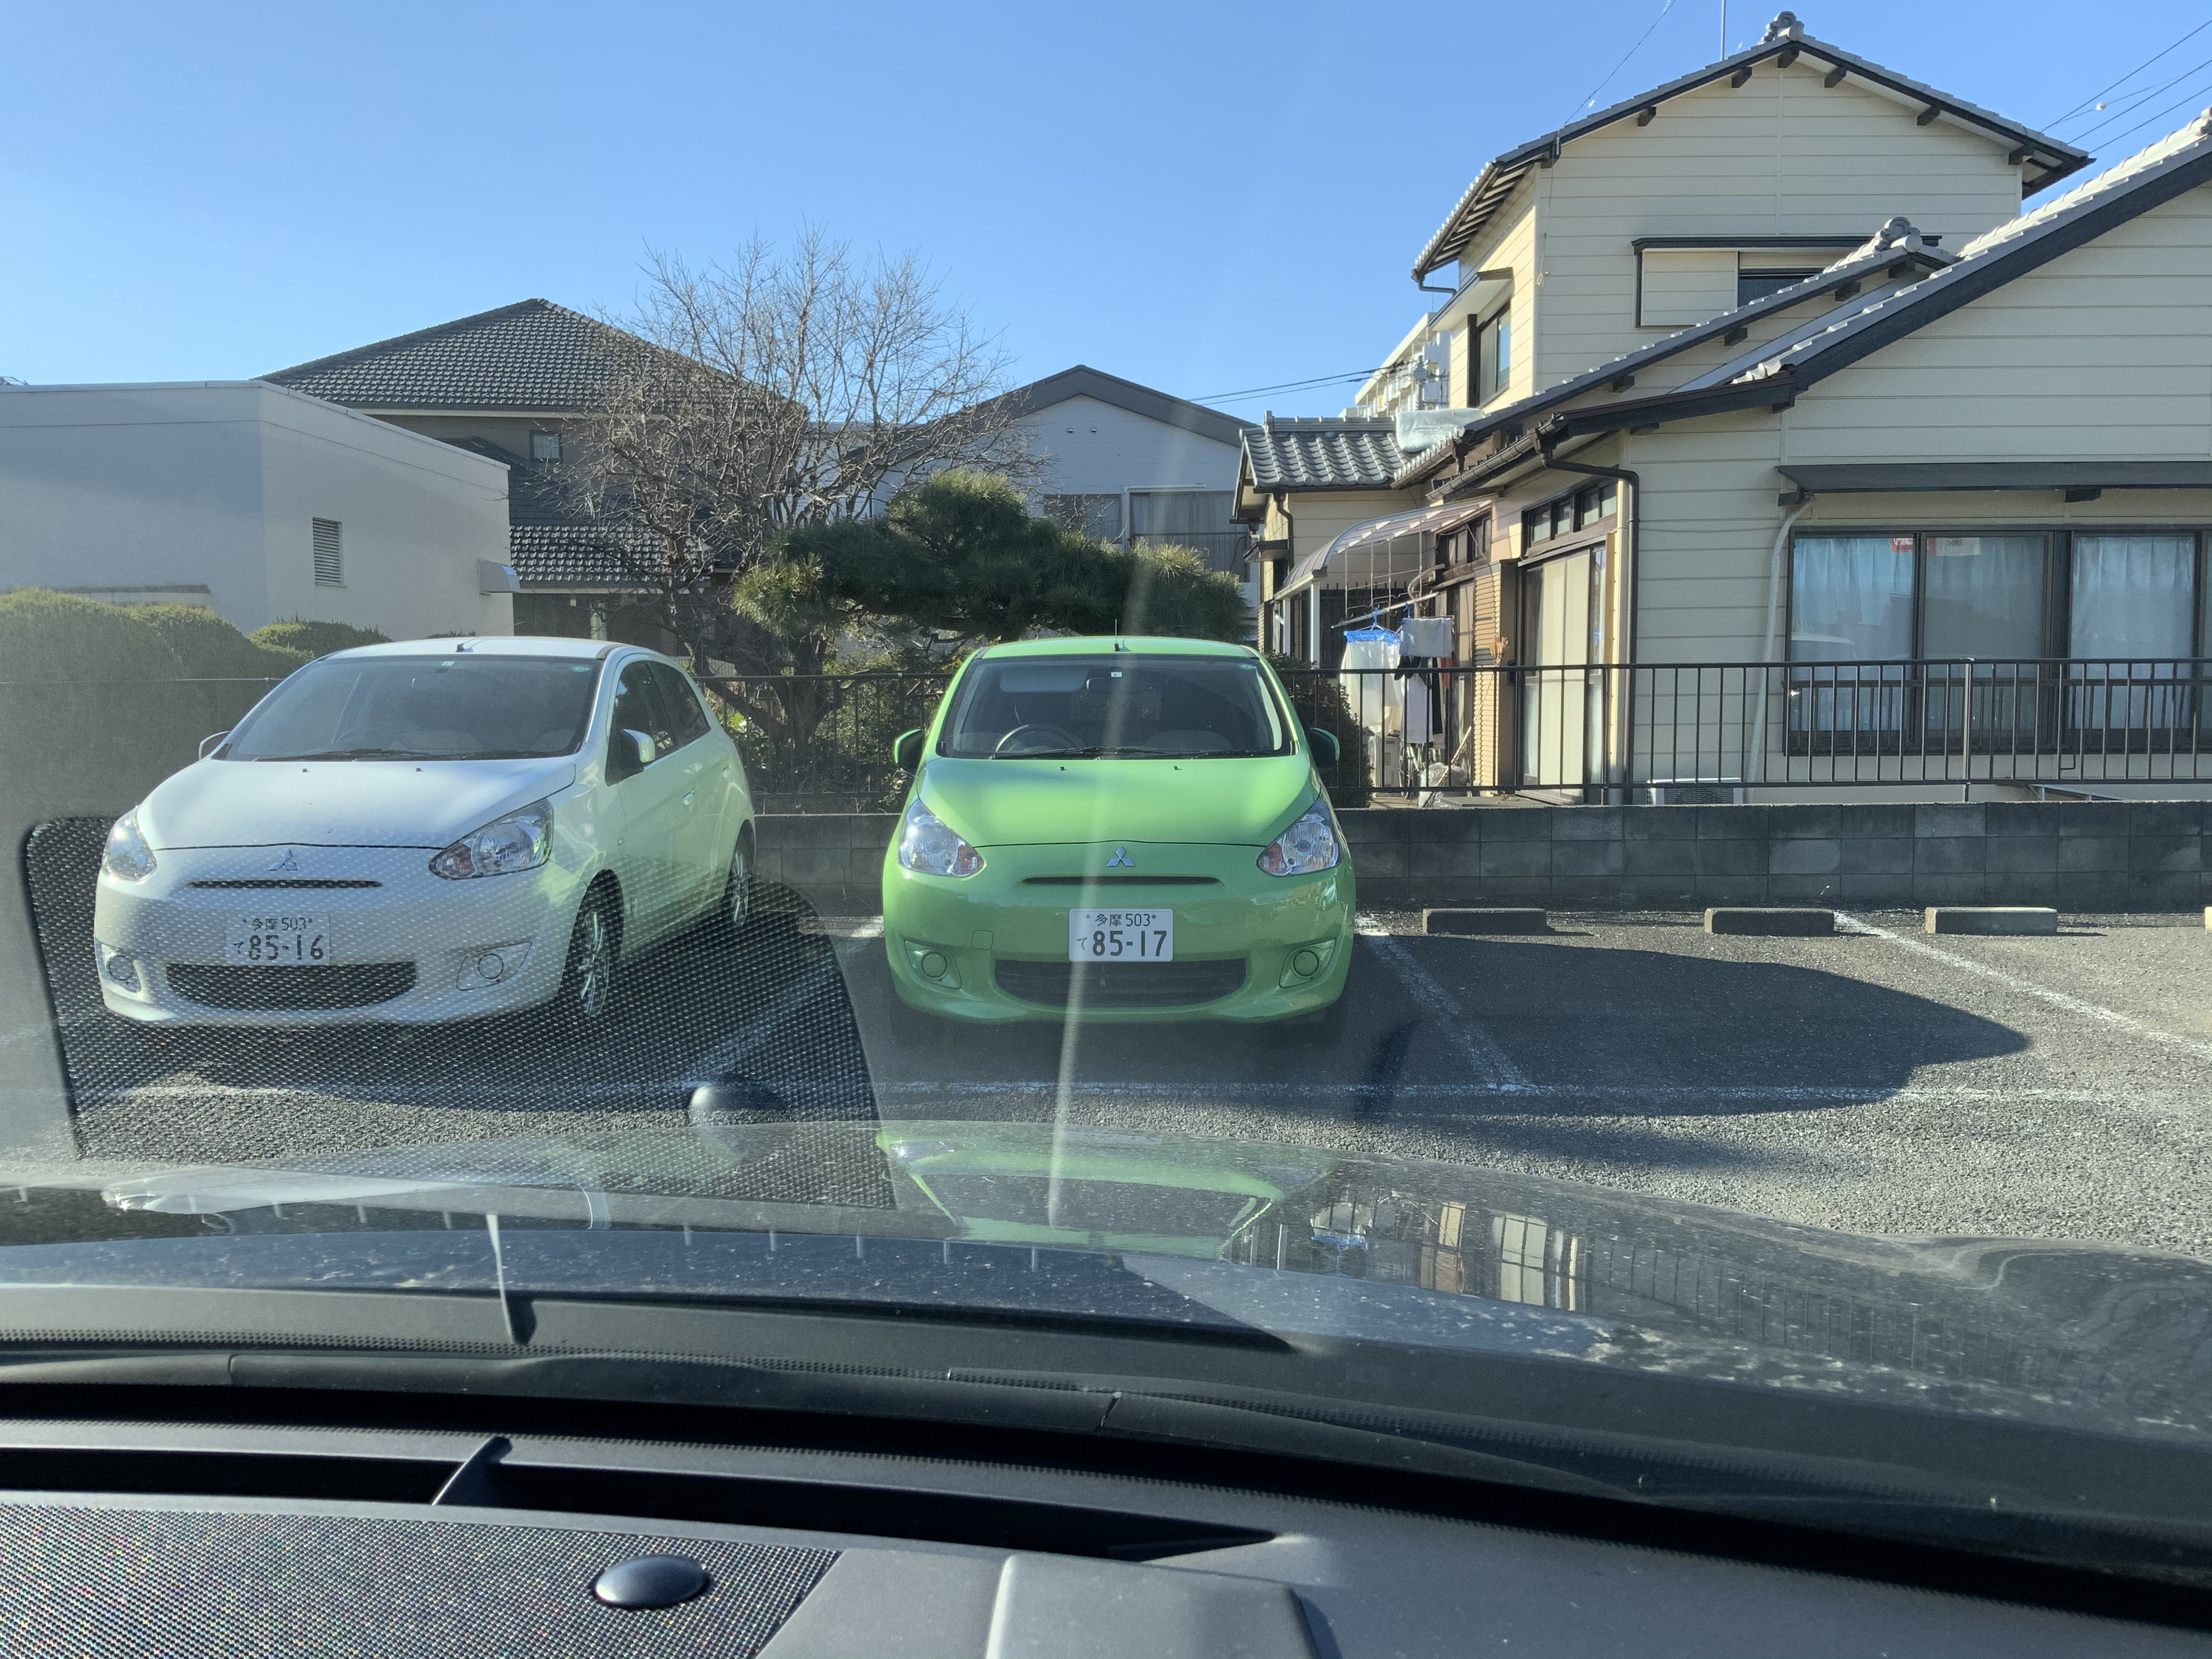
\includegraphics[width=4.5cm]{figs/sumple/4m_01.png}
    \end{center}
  \caption{車間距離4m}
  \label{fig:sumple4}
\end{minipage}

  \begin{minipage}{0.33\hsize}
  \begin{center}
    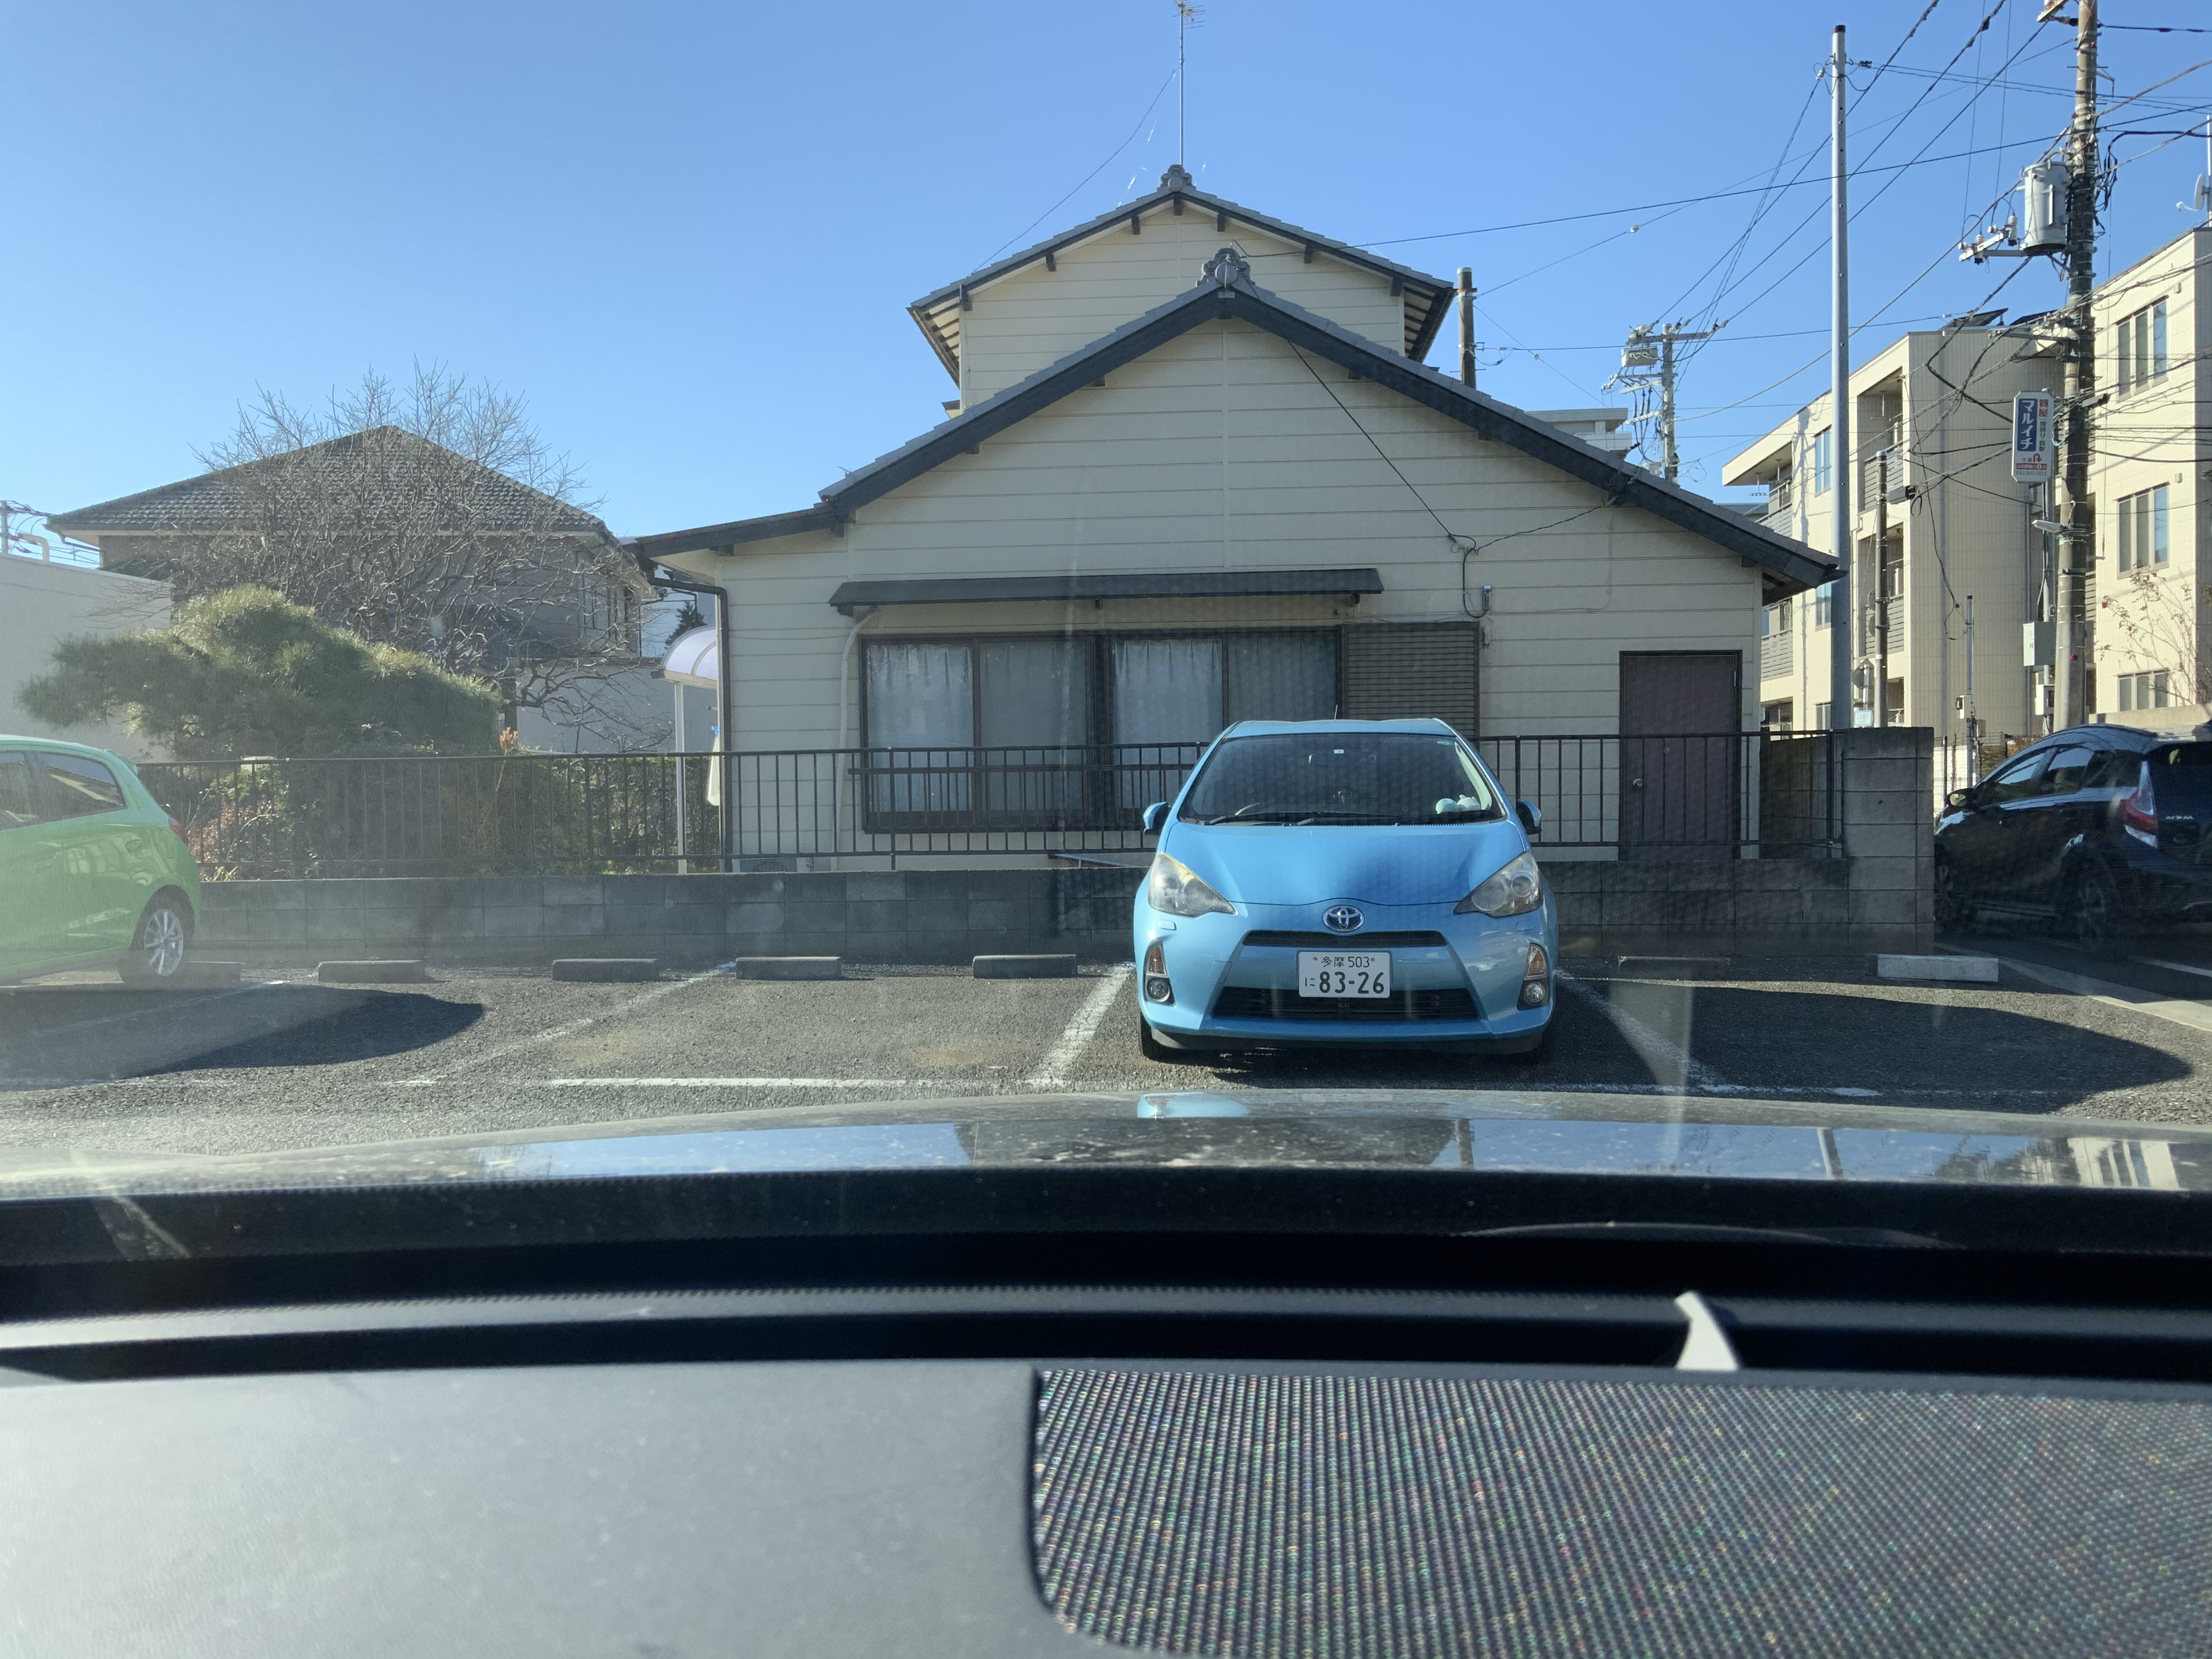
\includegraphics[width=4.5cm]{figs/sumple/5m_02.png}
  \end{center}
  \caption{車間距離5m}
  \label{fig:sumple5}
\end{minipage}

  \begin{minipage}{0.33\hsize}
  \begin{center}
    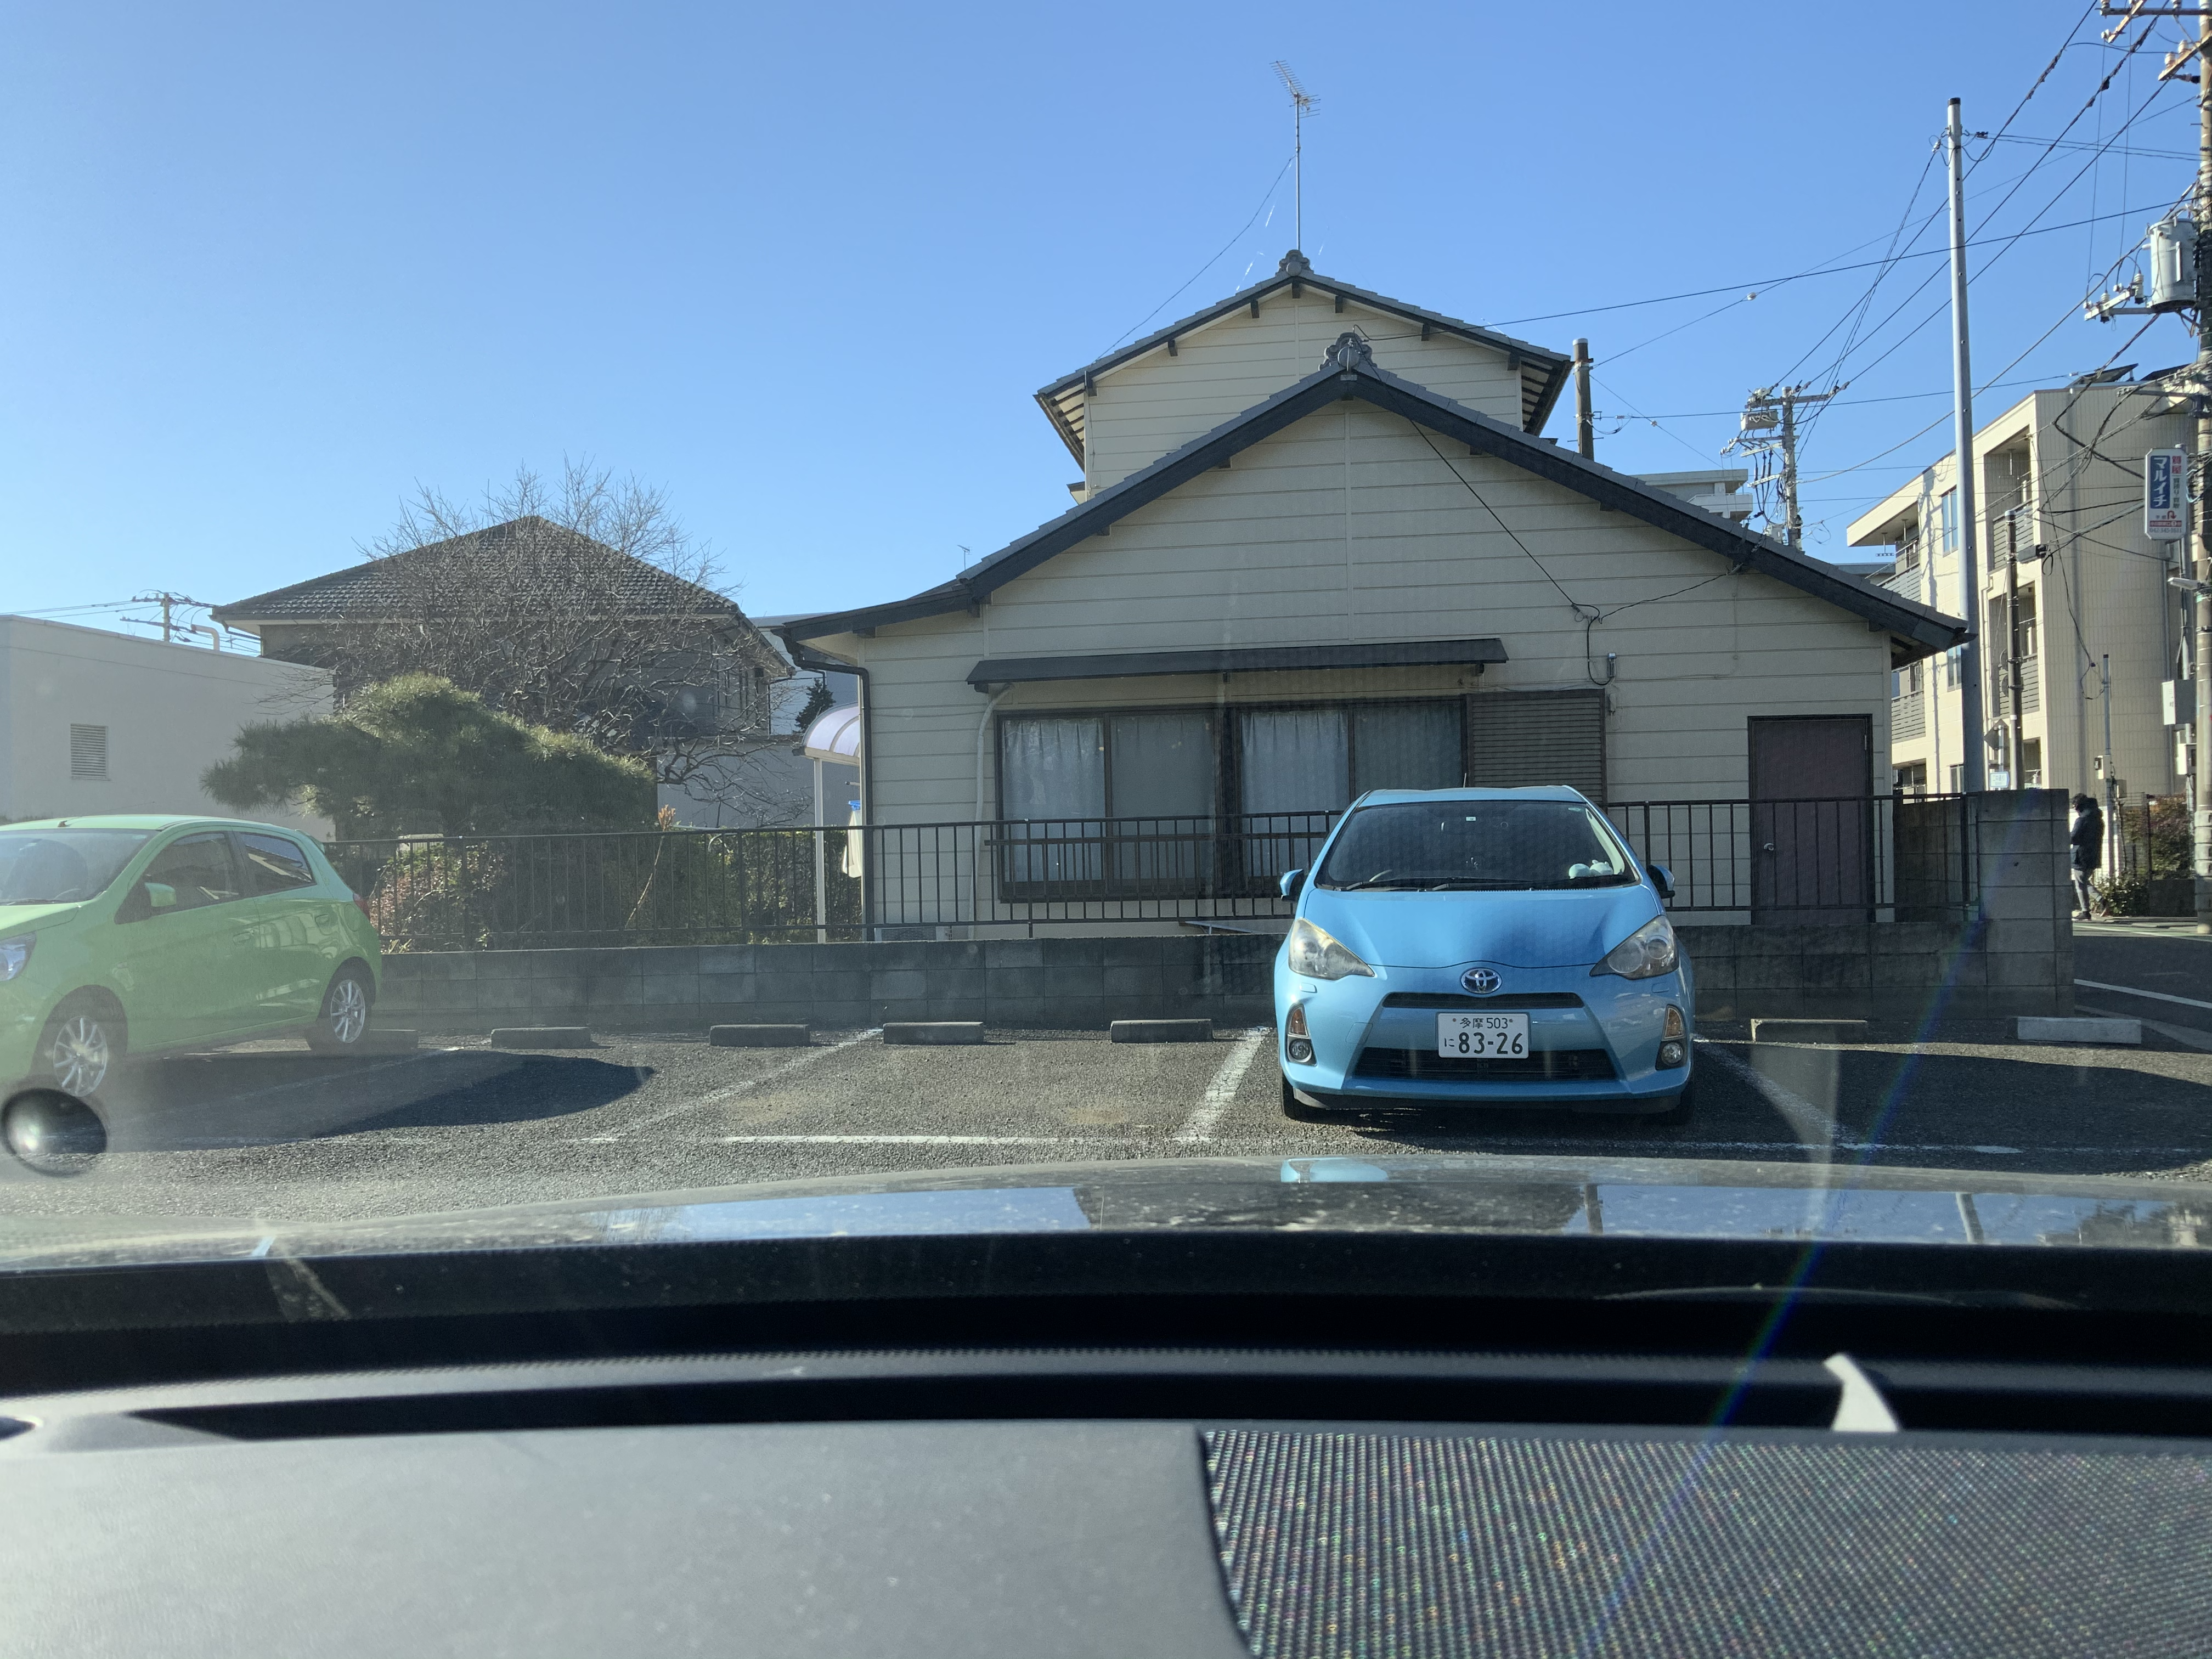
\includegraphics[width=4.5cm]{figs/sumple/6m_01.png}
  \end{center}
  \caption{車間距離6m}
  \label{fig:sumple6}
\end{minipage}
\end{tabular}
\end{figure}

% ---------------------------------------------------

上記の項で示したサンプルデーターをstruct2depth及びYoloシステムを利用して,それぞれの距離においてstrct2depthの数値がどのように変わるかを調べた.
その際,OpenCVの色情報取得システムを利用し,また検出されたBOXの中においてRGB値それぞれの最大値と平均値を比較しどちらを利用すると良いかについても調べた.

\subsection{実験結果}

% ------------------------------------------------------------

\begin{figure}[htbp]
  \begin{tabular}{c}
    \begin{minipage}{0.33\hsize}
      \begin{center}
   \includegraphics[width=4.5cm]{figs/sumple/4m_02mean.png}
    \end{center}
  \caption{車間距離4m時の平均値}
  \label{fig:sumple4mean}
\end{minipage}

  \begin{minipage}{0.33\hsize}
  \begin{center}
    \includegraphics[width=4.5cm]{figs/sumple/5m_02mean.png}
  \end{center}
  \caption{車間距離5m時の平均値}
  \label{fig:sumple5mean}
\end{minipage}

  \begin{minipage}{0.33\hsize}
  \begin{center}
    \includegraphics[width=4.5cm]{figs/sumple/6m_01mean.png}
  \end{center}
  \caption{車間距離6m時の平均値}
  \label{fig:sumple6mean}
\end{minipage}
\end{tabular}
\end{figure}

% ------------------------------------------------------------

\begin{figure}[htbp]
  \begin{tabular}{c}
    \begin{minipage}{0.33\hsize}
      \begin{center}
   \includegraphics[width=4.5cm]{figs/sumple/4m_02max.png}
    \end{center}
  \caption{車間距離4m時の最大値}
  \label{fig:sumple4max}
\end{minipage}

  \begin{minipage}{0.33\hsize}
  \begin{center}
    \includegraphics[width=4.5cm]{figs/sumple/5m_02max.png}
  \end{center}
  \caption{車間距離5m時の最大値}
  \label{fig:sumple5max}
\end{minipage}

  \begin{minipage}{0.33\hsize}
  \begin{center}
    \includegraphics[width=4.5cm]{figs/sumple/6m_01max.png}
  \end{center}
  \caption{車間距離6m時の最大値}
  \label{fig:sumple6max}
\end{minipage}
\end{tabular}
\end{figure}

% ---------------------------------------------------

また,画像の中のR値とG値を\tabref{tab:mean_max}に示す.その際,扱う数値は画面中央に近い自動車の検出された値とする.

% ----------------------------------------------------
\begin{table}[htbp]
  \centering
  \begin{scriptsize}
  \begin{tabular}{ccccccc}
  \toprule
& & 平均値 & 最大値 & & 平均値 & 最大値 \\
  \midrule
4m & R値 & 226.75 & 253.00 & G値 & {\bf129.54} & 203.00 \\
5m & R値 & 213.53 & 249.00 & G値 & {\bf 110.19} & 153.00 \\
6m & R値 & 201.77 & 253.00 & G値 & {\bf 97.33} & 201.00\\
  \bottomrule
  \end{tabular}
  \end{scriptsize}
  \caption{距離別の平均値と最大値}
  \label{tab:mean_max}
\end{table}
% ------------------------------------------------------

\subsection{評価基準の作成}
\label{sec:hyoukakijun}
\tabref{tab:mean_max}からわかることはR値は平均値と最大値のどちらにおいても距離との相関関係は薄いが,G値の特に平均値は距離が近くなるにつれて値が大きくなる傾向があるということである.
この実験結果をもとに,今後の実験においてはG値の平均値を用い,また予備実験3の実験内容の項で述べた通り,車間距離5mを基準とし,G値が100を下回った際に渋滞していると判断する.

\section{ドライブレコーダー映像を用いた予備実験}
\subsection{実験内容}
作成された評価基準を用いて実際にDepth2Jamがどのようなパフォーマンスをするか検証する実験を行った.
\ref{sec:hyoukakijun}の通り,strct2depth画面における車のbbox内のG値が100を超えた際に渋滞と判断し,画面左上に「Traffic Jam」という文字列が表示されるようにした.
加えて,映像中に渋滞が判断された回数をフレームごとにJam Counterとして回数を映像中段左に表示されるようにした.

\subsection{使用したデータセット}
本実験にて使用したデータセットは動画投稿サイトYouTubeにて公開されていた高速道路を走行中の映像に加え,私の家族が使用している自家用車に取り付けられたドライブレコーダー映像を用いる.
どの映像も30秒から1分のものであり,常に先行車がある映像を使用した.以下に使用した映像について表で示す.

% ----------------------------------------------------
\begin{table}[htbp]
  \centering
  \begin{scriptsize}
  \begin{tabular}{ccccc}
  \toprule
映像番号 & 時間帯 & 撮影場所 & 車線数 & 動画時間\\
  \midrule
映像1 & 昼間 & 一般道 & 1 & 60秒\\
映像2 & 昼間 & 一般道 & 2 & 60秒\\
映像3 & 不明 & 高速道路(トンネル) & 2 & 60秒 \\
  \bottomrule
  \end{tabular}
  \end{scriptsize}
  \caption{使用したデータセット}
  \label{tab:dataset}
\end{table}
% ------------------------------------------------------

\section{実験結果と課題}
\label{sec:kadai}
予備実験にて改良したシステムをそのまま用いると,様々な状況で渋滞を誤検出するという問題が発生してした.
誤検出の例を\figref{fig:ex01_01},\figref{fig:ex01_02},\figref{fig:ex01_03}に示す.

% --------------------------------------------------
\begin{figure}[htbp]
  \begin{tabular}{c}
    \begin{minipage}{0.33\hsize}
      \begin{center}
   \includegraphics[width=4.5cm]{figs/ex01_01.png}
    \end{center}
  \caption{結果1}
  \label{fig:ex01_01}
\end{minipage}

  \begin{minipage}{0.33\hsize}
  \begin{center}
    \includegraphics[width=4.5cm]{figs/ex01_03.png}
  \end{center}
  \caption{結果2}
  \label{fig:ex01_02}
\end{minipage}

  \begin{minipage}{0.33\hsize}
  \begin{center}
    \includegraphics[width=4.5cm]{figs/ex01_02.png}
  \end{center}
  \caption{結果3}
  \label{fig:ex01_03}
\end{minipage}
\end{tabular}
\end{figure}
% ---------------------------------------------------

\figref{fig:ex01_01},\figref{fig:ex01_02},および\figref{fig:ex01_03}の結果からわかるように様々な要因で渋滞の誤検出が起きた.
まず,\figref{fig:ex01_01}においては対向車がドライブレコーダー付きの自動車を横切ってしまうとその際に渋滞と判断してしまう例である.
対向車の存在は渋滞と関係ないのに対し,渋滞と判断してしまうのは正しい判断ではない.
次に,\figref{fig:ex01_02}においては,道路脇に駐車しているトラックを画像検知システムが検知してしまい,渋滞だと判断している例である.
高速道路では稀であるが一般道を走行している際に道路脇に自動車が駐車されているのは珍しいことではなく,またその駐車は渋滞には一切関係がない.
それにもかかわらず渋滞だと判断しているのは正しい判断ではない.
そして,\figref{fig:ex01_03}においては,複数車線がある場合に隣の車線の自動車が近くで走行している際に渋滞だと判断してしいる例である.
先述の対向車のケースとは異なり,隣の車線の混雑は走行車線の混雑と関係がある.
しかし,\figref{fig:ex01_02}のように,先行車との距離があるにもかかわらずたまたま隣で走っていたトラックが近いがために渋滞だと判断してしまうのは正しい判断ではない.
これらの判断ミスのケースは\tabref{tab:dataset}の表にある映像のいずれにおいても頻繁に発生する問題であった.

\newpage
\section{Depth2Jamの改良}
問題への解決アプローチとして,検出する自動車を絞る手法をとった.
対向車,隣車線の自動車および駐車している自動車を検出しないようにした.
対向車や隣車線の自動車といったものはドライブレコーダー映像において左右の1/3に写っていることが多いため,左右1/3に写っている自動車類の検出をしないように改良した.

プログラムにおいて処理中の画像の横のサイズは416ピクセルなので,その1/3である138ピクセルの範囲で左右における自動車類を検出しないようにした.

\section{実験結果}
映像中における実験1と同じフレームの画像での実験結果を以下に示す.

% --------------------------------------------------
\begin{figure}[htbp]
  \begin{tabular}{c}
    \begin{minipage}{0.33\hsize}
      \begin{center}
   \includegraphics[width=4.5cm]{figs/ex01_01after.png}
    \end{center}
  \caption{結果1}
  \label{fig:ex01_01after}
\end{minipage}

  \begin{minipage}{0.33\hsize}
  \begin{center}
    \includegraphics[width=4.5cm]{figs/ex01_03after.png}
  \end{center}
  \caption{結果2}
  \label{fig:ex01_02after}
\end{minipage}

  \begin{minipage}{0.33\hsize}
  \begin{center}
    \includegraphics[width=4.5cm]{figs/ex01_02after.png}
  \end{center}
  \caption{結果3}
  \label{fig:ex01_03after}
\end{minipage}
\end{tabular}
\end{figure}
% ---------------------------------------------------

\figref{fig:ex01_01after},\figref{fig:ex01_02after}および\figref{fig:ex01_03after}からわかる通り,左右の1/3を検出しないことで先行車のみを検出し,より正しく渋滞推定を行うことができている.
また,実験1と実験2における動画の中で渋滞だと検出した回数の比較の表を以下に示す.

% ----------------------------------------------------
\begin{table}[htbp]
  \centering
  \begin{scriptsize}
  \begin{tabular}{ccc}
  \toprule
映像番号 & 実験1 & 実験2\\
  \midrule
映像1 & 425 & 131\\
映像2 & 1309 & 401\\
映像3 & 256 & 59\\
映像4 & 1364 & 65\\
  \bottomrule
  \end{tabular}
  \end{scriptsize}
  \caption{実験2 - 結果}
  \label{tab:dataset}
\end{table}
% ------------------------------------------------------

\section{まとめ}
本章では,本研究におけるシステムの実装とシステム改良のための予備実験について述べた.
予備実験では使用する深度推定ライブラリの決定,画像圧縮問題の解決および評価基準の決定を行った.
次章では本研究における本実験について述べる.
\chapter{実験}
ここでは本研究において行った実験について述べる.

\section{さまざまな状況における本システムの推定精度実験}
実装と予備実験の項で述べた実験を通してシステムをさらに改良し,さまざまな状況下のドライブレコーダー映像を使って本システムの推定精度を測定する実験を行った.
これまでの実験に用いたデーターセットはどれも前方に先行車があるという状況だったが,この実験では先行車がない映像や信号で停止している映像を用いて本システムの推定精度に関して実験評価を行う.
実験3を行うにあたって人間の目で渋滞しているフレーム数を数える必要があるため,システムにおいて出力された映像の中央にフレーム数を明記されるように改良した.
また,本実験においては人間の目で渋滞を判断するにあたって,信号等の要素を排除し,車道において先行車が停止し,停止ランプがついており,ドライブレコーダーが取り付けられている自動車も停車している状況を渋滞と判断した.
%
%そのうえで,この実験が提案手法を評価する上で十分なのか,もう少し検討しましょう.
%少なくとも,各動画の渋滞状況をground truthとして示し,システムでの検出結果を示し,それらを比較する必要があります.
%これに加えて,全く渋滞していない,少し流れが悪い,断続的に渋滞,全く動いていない,みたいに,いろいろな状況の動画での実験が必要と思います.
%
%

\subsection{使用したデータセット}
本実験において使用したデータセットを以下の表に示す.

% ----------------------------------------------------
\begin{table}[htbp]
  \centering
  \begin{scriptsize}
  \begin{tabular}{cccccc}
  \toprule
映像番号 & 映像の内容 & 映像時間 & フレーム数 & 時間帯 & 道路 \\
  \midrule
映像1 & 全く渋滞していない & 60秒 & 1830フレーム & 昼 & 一般道 \\
映像2 & 先行車あり スムーズに進んでいる & 60秒 & 1830フレーム & 昼 & 一般道 \\
映像3 & 途中信号による停車あり & 60秒 & 1830フレーム & 昼 & 一般道 \\
映像4 & 渋滞中の継続的な渋滞 & 60秒 & 1830フレーム & 昼 & 一般道 \\
映像5 & 信号による停車 & 31秒& 928フレーム & 昼 & 一般道 \\
  \bottomrule
  \end{tabular}
  \end{scriptsize}
  \caption{実験3 データーセット}
  \label{tab:exp_dataset3}
\end{table}
% ------------------------------------------------------

\subsection{結果}
上記のデータセットを使い,本システムの推定精度を実験した.
また出力された数値をもとにmAP(mean Average Precision)値を求め,以下に示す.

% ----------------------------------------------------
\begin{table}[htbp]
  \centering
  \begin{scriptsize}
  \begin{tabular}{cccc}
  \toprule
映像番号 & 映像の内容 & システムの渋滞推定フレーム数 & 渋滞判断フレーム数(Ground Truth)\\
  \midrule
映像1 & 先行車なし 無渋滞 & 0 & 0 \\
映像2 & 先行車あり スムーズに進んでいる & 4 & 0 \\
映像3 & 途中信号による停車あり & 167 & 870\\
映像4 & 渋滞中の継続的な渋滞 & 130 & 452\\
映像5 & 信号による停車 & 251 & 927 \\
\bottomrule
\end{tabular}
\end{scriptsize}
  \caption{実験3 - 結果}
  \label{tab:exp3_fig}
\end{table}
% ------------------------------------------------------

\section{再現性 適合率 mAP}
本システムにおける再現性,適合率及びmAP値を測定するための実験を行った.
実験3にて出力された映像データー5つから,それぞれ20フレームずつ抽出し,合計100フレーム画像において,本システムの渋滞判断における再現性,適合率,mAPの値を調べた.
その結果を以下に示す.


\section{精度の考察}
画面全体を検出した場合の表\tabref{tab:mAP_fig_noweght}と\tabref{tab:mAP_fig}を比較する.
2つの表を比較した際に,大きな違いはFPである.実装したDepth2Jamは画面中央部分のみを検出するように改良したためFPがどの動画においても0という結果になっているが,画面全体を検出する場合ではFPが最大で29まで増加している.
画面両端の1/3部分を検出しないようにした結果,Depth2Jamの正確性が向上したことがこの比較でわかる.
次に,映像5における2つの結果を比較した際に,\tabref{tab:mAP_fig_noweght}においてはF値が0.82と\tabref{tab:mAP_fig}におけるF値の0.33より大幅に上昇している.

\subsection{誤検出}
まず,\ref{sec:exp1}における誤検出の例とその原因についての考察を述べる.
\tabref{tab:exp3_fig}において,映像1においては誤推定されたフレームは存在しないが,映像2においては渋滞ではないのに渋滞だと誤推定されたフレームが存在する.
誤推定されたフレームの例を\figref{fig:mov2miss01}と\figref{fig:mov2miss02}に示す.

% ---------------------------------
\begin{figure}[htbp]
  \begin{minipage}{0.5\hsize}
   \begin{center}
    \includegraphics[width=7cm]{figs/mov2miss/miss01.png}
   \end{center}
   \caption{誤検出の例1}
   \label{fig:mov2miss01}
  \end{minipage}
  \begin{minipage}{0.5\hsize}
  \begin{center}
   \includegraphics[width=7cm]{figs/mov2miss/miss02.png}
  \end{center}
   \caption{誤検出の例2}
   \label{fig:mov2miss02}
  \end{minipage}
 \end{figure}
% ---------------------------------

どちらのフレーム画像においても検出された自動車が中央に寄っており,かつ検出されたBBOXにおける平均G値が100を超えてしまっているので渋滞だと判断してしまっていることがわかる.
実装したDepth2Jamシステムにおいては,画面左右1/3における自動車の検出がされないようにしているが,この検出除外処理は,検出されたBBOXにおける2つのX軸の値のうち,左側つまり小さい方の値のX軸が画面の左右1/3の範囲に含まれる場合に発生する.
このフレームではそのX軸の値が中央1/3の範囲に含まれているためこのような結果になったのだと思われる.
より精度を向上させるために,BBOXにおけるX軸の値のうち,右側つまり値の大きい方のX軸に対しても追加で検出除外処理を設ける必要があると考えられる.

\newpage
\subsection{FNに関する考察}
ここでは,\tabref{tab:mAP_fig}におけるFNに関する考察について述べる.
映像1と映像2に関しては渋滞しているフレームは存在しないのでFNの値も0となっているが,映像3~5および総合においてはFNの値が目立つ.
FNはシステムが渋滞でないと判断したが,実際には渋滞していたフレームであり,現実では信号や渋滞等で自動車が動いていないのにシステムが渋滞だと判断できていなかったフレームである.
そのフレームの例を\figref{fig:fn01}と\figref{fig:fn02}に示す.

% ---------------------------------
\begin{figure}[htbp]
  \begin{minipage}{0.5\hsize}
   \begin{center}
    \includegraphics[width=7cm]{figs/consider/fn01.png}
   \end{center}
   \caption{FNの例1}
   \label{fig:fn01}
  \end{minipage}
  \begin{minipage}{0.5\hsize}
  \begin{center}
   \includegraphics[width=7cm]{figs/consider/fn02.png}
  \end{center}
   \caption{FNの例2}
   \label{fig:fn02}
  \end{minipage}
 \end{figure}
% ---------------------------------

どちらの例も先行車が停車しており,ドライブレコーダーを搭載した自動車も停車している状況である.
そして,検出されたBBOXにおいて,G値の値は70程度となっており,渋滞と判断されていない.
考えられる原因としてはドライバーが車間距離に余裕を持って停車しているため,G値が相対的に小さくなってしまっていることにあると考えられる.
車間距離に余裕を持って停車することは本来推奨される運転のため,余裕を持って車間距離をとっている場合でも渋滞だと推定できる手法を取る必要がある.


\section{結論}
% ほぼtanimuさんのパクリ
ここでは本研究における結論について述べる.
本研究ではドライブレコーダー及び深度推定ライブラリ,物体検出ライブラリを用いた渋滞推定システムDepth2Jamについての提案を行った.
深度推定ライブラリを用いることでカメラからの距離を推量することが可能であり,物体検出ライブラリを用いることで推量したい物体を検出することが可能である.
実験では実際にドライブレコーダー映像をもとに本研究を通して開発したシステムを用いて実証実験を行い,渋滞を推定できているか評価を行った.
本提案手法を通じて今まで設置されたものの実際の活用が少なかったドライブレコーダーがより活用されることが期待される.

% footer
\chapter*{謝辞}
本研究を進めるにあたり,ご指導を頂きました慶應義塾大学環境情報学部教授中澤仁博士に深く感謝いたします.また,慶應義塾大学中澤研究室の諸先輩方には折りに振れ貴重なご助言を頂きました.特に慶應義塾大学大学院政策・メディア研究科陳寅特任助教,慶應義塾大学大学院政策・メディア研究科大越匡特任講師,には本論文を執筆するにあたってご指導頂きました.ここに深く感謝の意を表します
最後に,前大学での1.5年間,そこから海外への半年の留学,そして1年間の浪人を経ての慶應義塾大学での4年間の生活を支えてくださった家族に深く感謝いたします.

\begin{flushright}
2020年1月21日\\
李 広耀
\end{flushright}


\bibliographystyle{junsrt}
\bibliography{ref.bib}

\appendix
% \def\thesection{付録\Alph{section}}
% \input{append}

\end{document}